\documentclass[10pt,a4paper,oneside,fleqn]{report}
\usepackage{geometry}
\geometry{a4paper,left=20mm,right=20mm,top=1cm,bottom=2cm}
\usepackage[utf8]{inputenc}
%\usepackage{ngerman}
\usepackage{amsmath}                % brauche ich um dir Formel zu umrahmen.
\usepackage{amsfonts}                % brauche ich für die Mengensymbole
\usepackage{graphicx}
\setlength{\parindent}{0px}
\setlength{\mathindent}{10mm}
\usepackage{bbold}                    %brauche ich für die doppel Zahlen Darstellung (Einheitsmatrix z.B)
\usepackage[linktocpage={false}]{hyperref}


\usepackage{color}
\usepackage{titlesec} %sudo apt-get install texlive-latex-extra

\definecolor{darkblue}{rgb}{0.1,0.1,0.55}
\definecolor{darkred}{rgb}{0.55,0.2,0.2}

\titleformat{\chapter}[display]{\color{darkred}\normalfont\huge\bfseries}{\chaptertitlename\
\thechapter}{20pt}{\Huge}

\titleformat{\section}{\color{darkblue}\normalfont\Large\bfseries}{\thesection}{1em}{}
\titleformat{\subsection}{\color{darkblue}\normalfont\Large\bfseries}{\thesection}{1em}{}

% Notiz Box
\usepackage{fancybox}
\newcommand{\notiz}[1]{\vspace{5mm}\ovalbox{\begin{minipage}{1\textwidth}#1\end{minipage}}\vspace{5mm}}

\usepackage{cancel}


%\includegraphics[width=0.75\textwidth]{thepic.png}
\begin{document}
%\tableofcontents
\setcounter{chapter}{9}
\chapter{Elektronische Transporteigenschaften}

Bewegung der \(e^-\)-nen, effektive Masse.

\section{Elektronien als Wellenpakete}

Ausgedehnte Wellen \(\delta k\delta r > 1\)

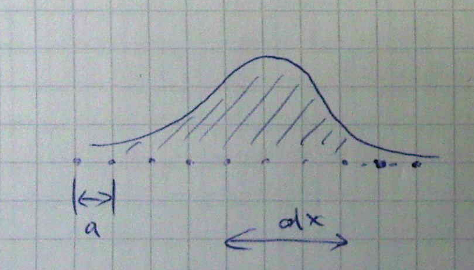
\includegraphics[width=0.75\textwidth]{kap10_01.png}

\[\psi(\vec r,t) = \sum_{\vec k} g(\vec k)\cdot e^{i(\vec k\vec r - \frac{\hbar k^2}{2m}t}\]

mit \(r= \frac{pt}{2m}\)

Koeffizienten \(g(\vec k)\) sind innerhalb \(\delta k\) 'gaußförmig' verteilt. Das entspricht einer semiklassischen Näherung. 

\[\frac{\partial \vec r}{\partial t} \equiv \vec v(\vec k) = \frac{1}{\hbar}\nabla_{\vec k}E(\vec k) = \frac{1}{\hbar} \frac{\partial E(\vec k)}{\partial \vec k} \]

mit \(E(\vec k) \) Energie vom Wellenpaket. z.B. für freie \(e^-\)-nen \(E=\frac{\hbar^2 k^2}{2m}\); \(v_g=\frac{\hbar k}{m}\) Gruppengeschwindikeit.

Semiklassische Bewegungsgleichung:

\[\hbar \frac{\partial \vec k}{\partial t}=\vec F = -e\vec \vec{ \mathcal E}(\vec r,t) -\vec v(\vec k)\times \vec B(\vec r,t)  \]

\(\vec{ \mathcal E}\) Elektrisches Feld; \(\vec B\) magnetisches Feld; \(E(\vec k) = E(-\vec k)\)

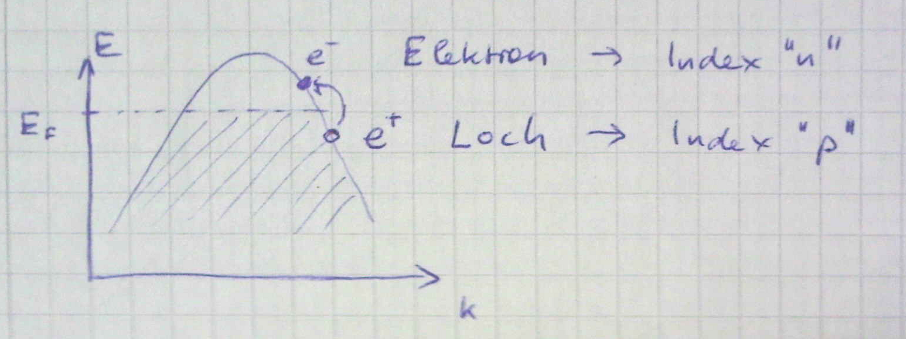
\includegraphics[width=0.75\textwidth]{kap10_02.png}

\(E_p(\vec k) = -E_n(\vec k)\)

Gruppengeschwindigkeit: \(\frac{\partial \vec v}{\vec t}(\frac{1}{\hbar}\frac{\partial E(\vec k)}{\partial \vec k})=\frac{\partial}{\partial \vec k}(\frac{1}{\hbar}\frac{\partial E(\vec k)}{\partial \vec k})\frac{d\vec k}{dt}=\frac{1}{\hbar^2}\vec F\frac{\partial^2 E(\vec k}{\partial \vec k\partial\vec k}\)

\[\frac{\partial v_i}{\partial t} = \frac{1}{\hbar}\sum_j \frac{\partial^2 E(\vec k)}{\partial k_i\partial_j}F_j\]

Tensor der effektive Masse \([m*]\equiv \stackrel{\mathrm{=}}m^* \)

mit 

\[\left(\frac{1}{m^*}\right)_{ij}=\frac{1}{\hbar^2}\frac{\partial^2 E(\vec k)}{\partial k_i\partial k_j}\]


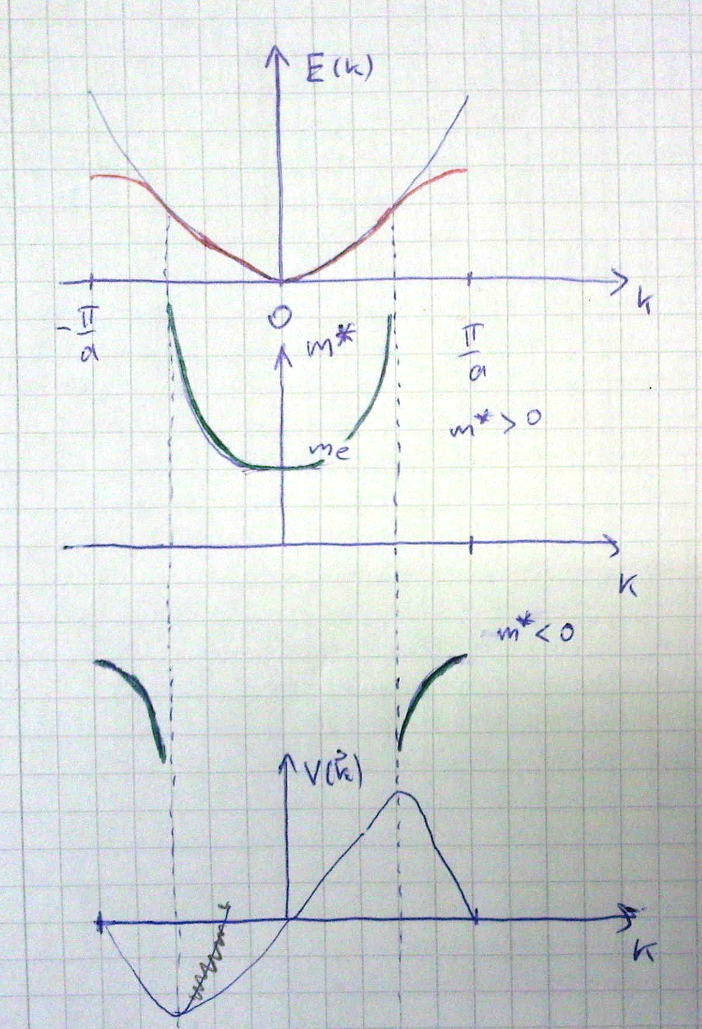
\includegraphics[width=0.75\textwidth]{kap10_03.png}

1D: \(m^*\) ist klalare Größe \(m^*(k) = \frac{\hbar^2}{[\frac{d^2E(k)}{dk^2}]}\)

Bloch-oszillationen: \(\hbar \frac{dk}{dt} = F = -e\mathcal E\)


Periode dieser Bloch Oszillationen:

\[T\propto \frac{\delta k}{|dk/dt|}\propto \frac{2\pi/a}{e\mathcal E/\hbar}\]


\end{document}
